\documentclass{beamer}

\usepackage{default}

\usepackage[danish]{babel}
\usepackage[utf8]{inputenc}
\usetheme[progressbar=frametitle]{metropolis}
\usepackage{appendixnumberbeamer}


\usepackage{booktabs}
\usepackage[scale=2]{ccicons}

% \usepackage{pgfplots}
% \usepgfplotslibrary{dateplot}

\usepackage{graphicx}

\definecolor{Orange}{RGB}{229,134,25}

\usepackage{xspace}
\newcommand{\themename}{\textbf{\textsc{metropolis}}\xspace}
\usepackage{listings}


\definecolor{background}{RGB}{226, 226, 226}


\lstset{ 
	literate=% 
	{Ö}{{\"O}}1 
	{Ä}{{\"A}}1 
	{Ü}{{\"U}}1 
	{ß}{{\ss}}{ 1\negmedspace\,} 
	{ü}{{\"u}}1 
	{ä}{{\"a}}1 
	{ö}{{\"o}}1 
	{ø}{{\o}}{1\negmedspace\,} 
	{Ø}{{\O}}{1\negthinspace\,\,} 
	{å}{{\aa}}{1\negthickspace\,} 
	{Å}{{\AA}}{1\negthinspace\,} 
	{æ}{{\ae}}{1\negthinspace\,} 
	{Æ}{{\AE}}{1\,\,}}

\lstdefinestyle{terminal}{
	language=bash,
	aboveskip=2mm,
	belowskip=2mm,
	showstringspaces=false,
	columns=flexible,
	basicstyle={\small\ttfamily},
	numbers=none,
	numberstyle=\footnotesize,
	commentstyle=\color{black},
	frame=single,
	framesep=2pt,
	breaklines=true,
	breakatwhitespace=false,
	backgroundcolor = \color{background},
	tabsize=2
}


\lstdefinestyle{python}{
	language=Python,
	aboveskip=2mm,
	belowskip=1mm,
	showstringspaces=false,
	columns=flexible,
	numbers=none,
	numberstyle=\footnotesize,
	commentstyle=\ttfamily\color{black},
	frame=single,
	framesep=2pt,
	breaklines=true,
	breakatwhitespace=false,
	backgroundcolor = \color{background},
	tabsize=2
}



\title{Lær Python dag 1 - modul 1}
\subtitle{Introduktion, basis python}
% \date{\today}
\date{}
\author{Jonas Bamse Andersen}
\institute{Syddansk Universitet}
%\titlegraphic{\hfill
\includegraphics[height=1.5cm]{logo.pdf}}

\begin{document}
	
	\maketitle

\begin{frame}{Hjemmeside}

Kurset har en hjemmeside: \url{https://jonan15.github.io/python-F19/}
\begin{center}
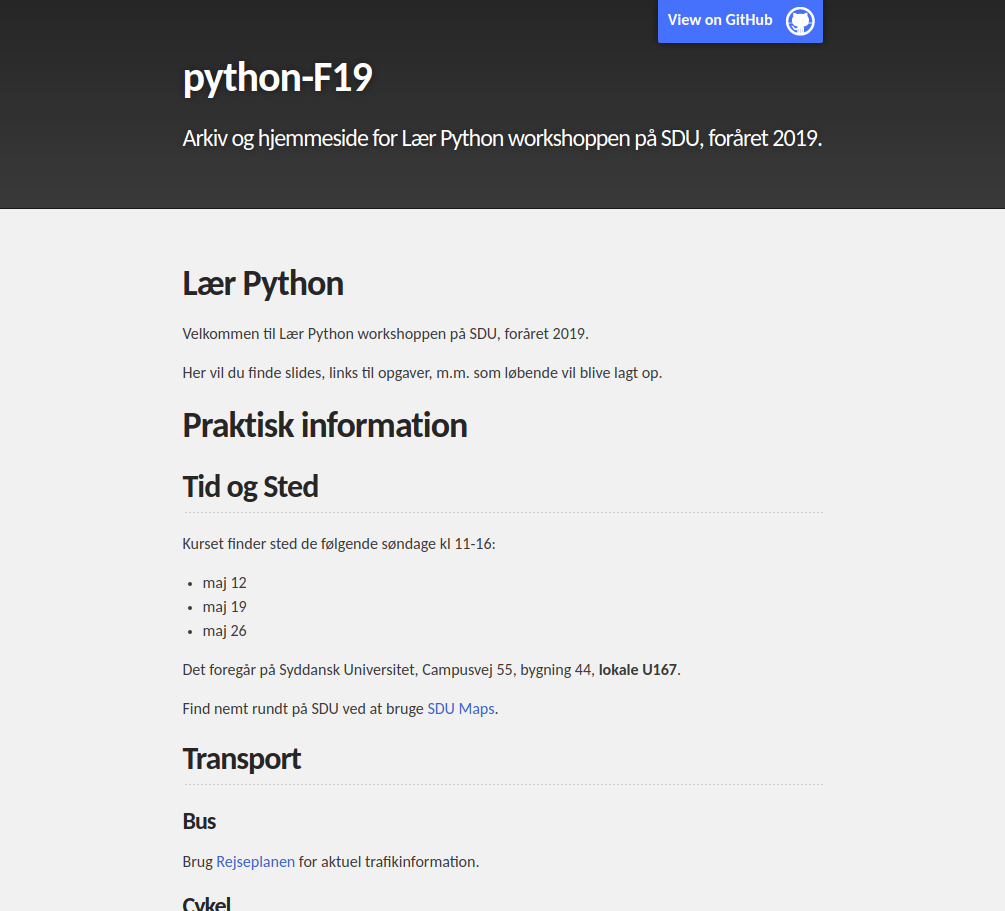
\includegraphics[trim={0 5cm 0 0}, clip, width=0.6\textwidth]{webpage.png}
\end{center}

Her findes slides, opgaver og eventuelle tips og tricks.	
\end{frame}


\begin{frame}{Colaboratory}
Online editor og interpreter (fortolker).

Kræver en Google Account.

\begin{center}
	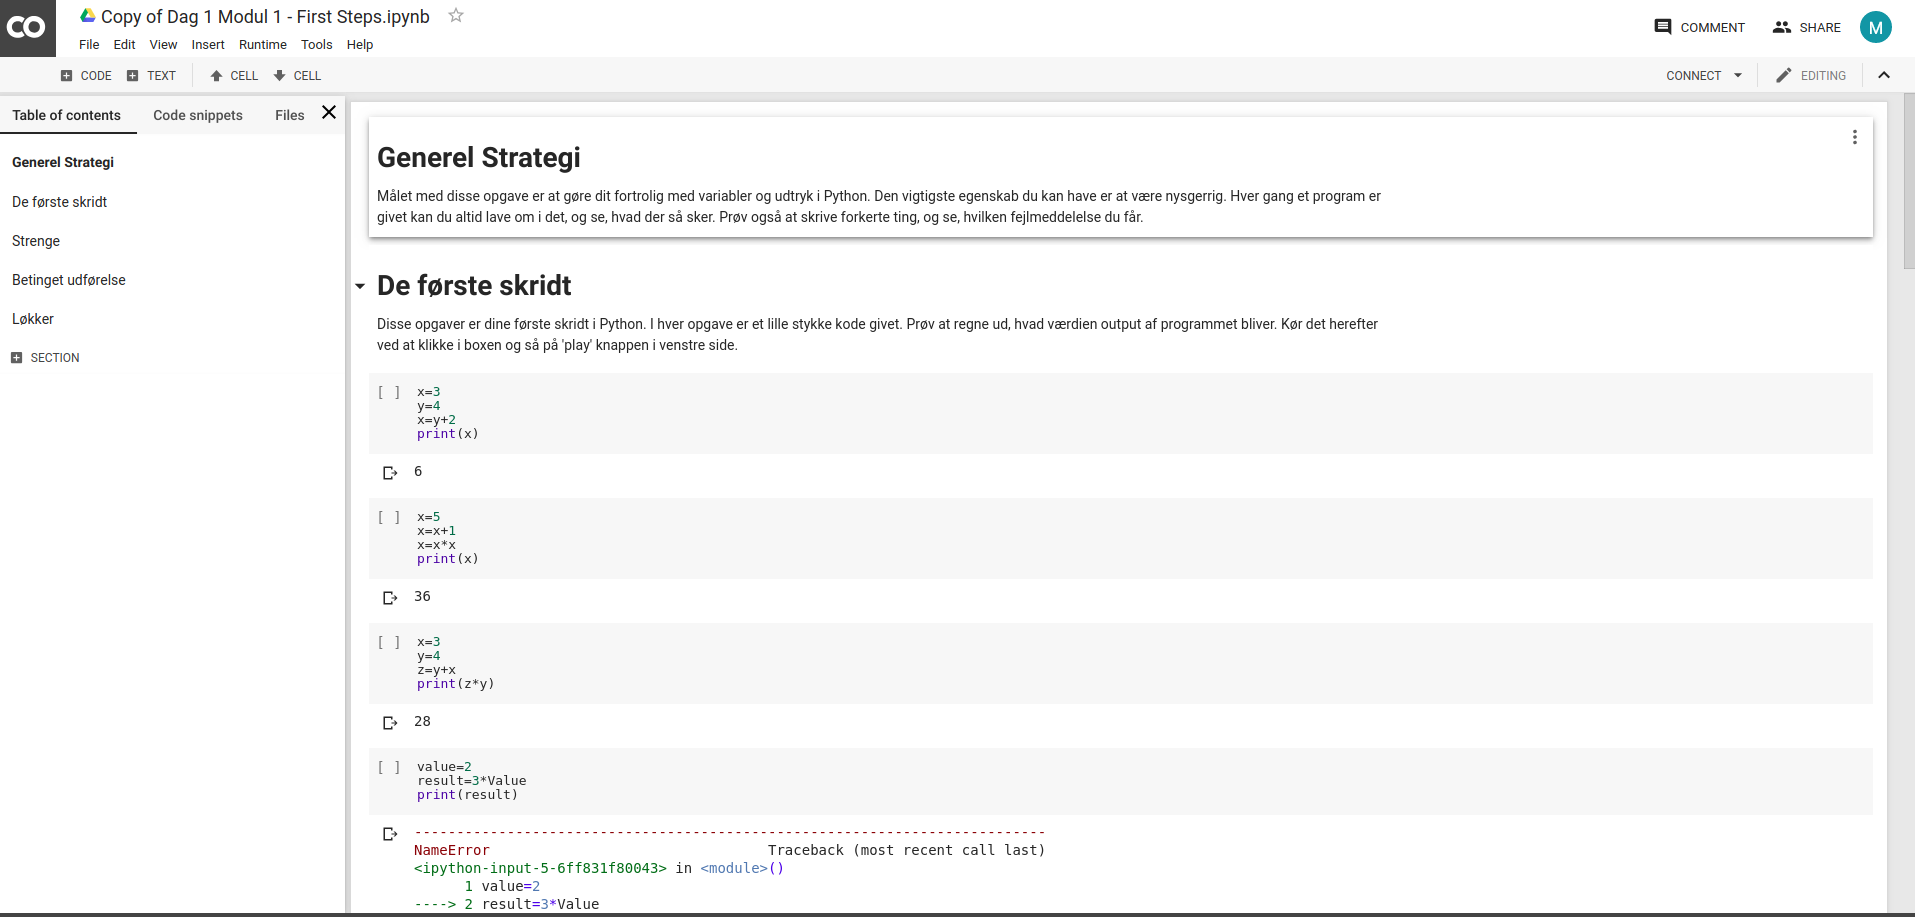
\includegraphics[width=\textwidth]{colaboratory.png}
\end{center}

Man kan også installere Python på sin egen computer.
\end{frame}

\begin{frame}{Hvad er Python?}
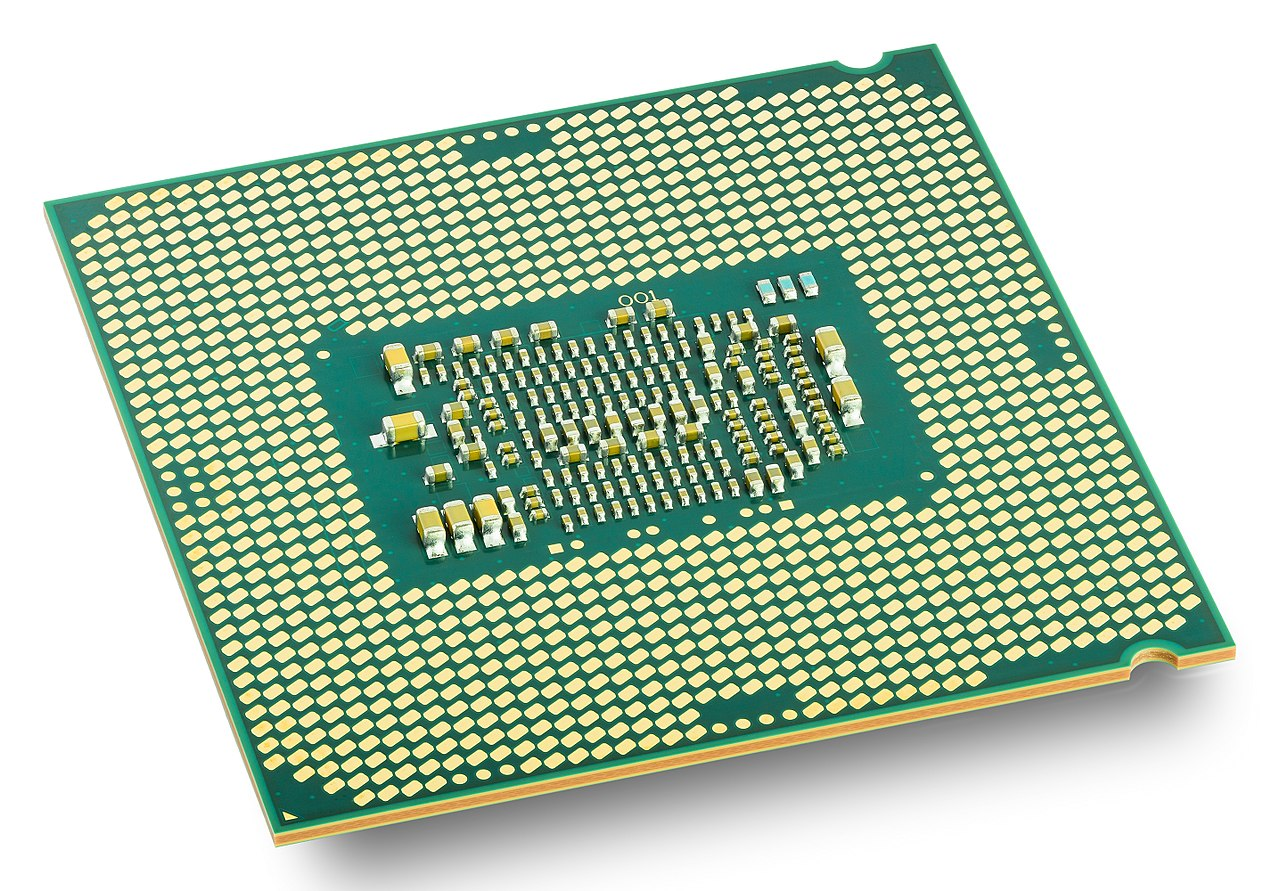
\includegraphics[width=\textwidth]{cpu.jpg}
\end{frame}



\begin{frame}{Hvad er Python?}
\begin{center}
\begin{columns}
	\column{0.4\textwidth}
	Hvad er en computer?
	\pause

	Hvad er et program?
	\pause

	Program = sekvens af instruktioner.
	\pause
	
	Computere er dumme! De gør kun som de får besked på...
	\pause

	\column{0.4\textwidth}
	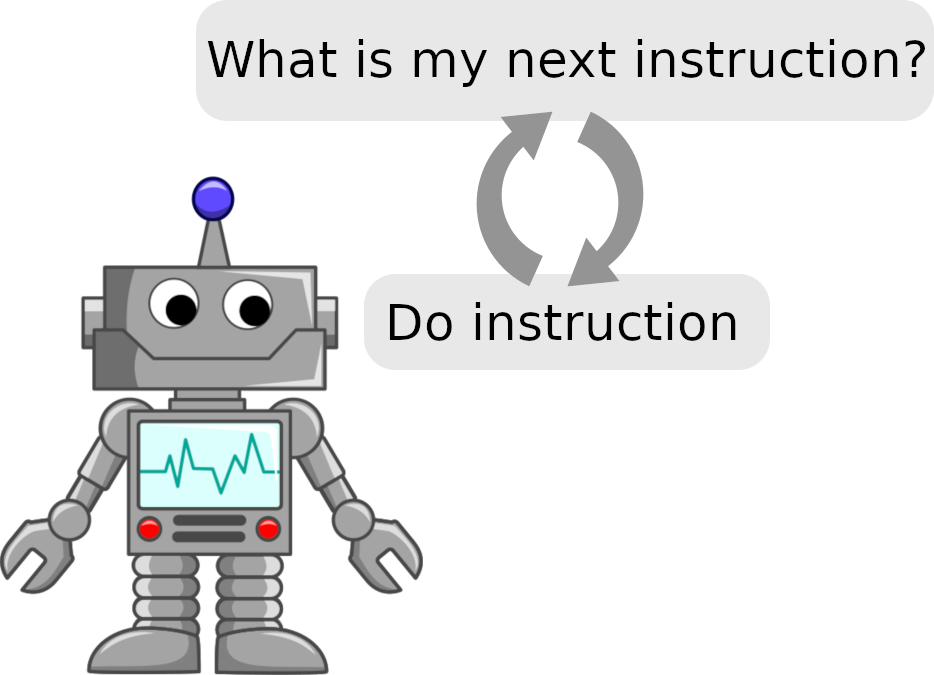
\includegraphics[width=\textwidth]{cpu-cartoon.png}
	\pause
	
	Tilgengæld er de lynende hurtige.
\end{columns}
\end{center}
\end{frame}



\begin{frame}{Hvad er Python?}
Python er et programmeringssprog.

Sproget bestemmer hvilke instruktioner man kan skrive.

Men sproget skal oversættes/fortolkes.

\pause
\begin{center}
\textbf{1 linje $\approx$ 1 instruktion. \\
	Programmet oversættes fra toppen og nedad.}
\end{center}
\end{frame}



\begin{frame}{Programmer}
Når vi snakker om programmer kan vi bl.a. snakke om:
\begin{itemize}
	\item Instruktioner: Hvad selve programmet består af.
	\pause
	\item Input: "Data" som programmet skal forholde sig til.
	\pause
	\item Output: Resultatet af programmet, f.eks. tekst/grafik på en skærm eller en ny fil.
\end{itemize}

\end{frame}



\begin{frame}{Fordele/Ulemper ved Python}
\metroset{block=fill}
\begin{exampleblock}{Fordele}
\begin{itemize}
\item Simpelt sprog - \textbf{nemt at lære}
\item Stort standardbibliotek (allerede implementerede funktioner)
\item Kan køre på mange platforme
\item Udbredt brugt både i industri og forskning
\end{itemize}
\end{exampleblock}

\begin{alertblock}{Ulemper}
\begin{itemize}
\item Langsommere end sprog som C/C++
\item Typer er uskrevne (dynamisk)
\end{itemize}
\end{alertblock}
\end{frame}




\begin{frame}{Hvad bruges Python til}
\begin{itemize}
\item Scripting - små hurtige programmer
\item Data behandling og visualisering
\item Machine Learning og Deep Learning
\item Backend-development (f.eks. brugt af Instagram)
\item Hardwareprojekter
\end{itemize}
\end{frame}

\section{Programmering i Python}

\begin{frame}[fragile]{Eksekvering i en terminal}
\begin{itemize}
\item Åben en terminal (mac), komandoprompt (windows)
\item Naviger til placering af dit python-program
\item Eksekver med følgende kommando:
\begin{lstlisting}[style=terminal]
python <program_navn>.py
\end{lstlisting}
\end{itemize}

\end{frame}

\begin{frame}{Eksekvering i pycharm}
Tryk på play-knappen.
\begin{center}
\includegraphics[width=\textwidth]{figures/eksekvering_pycharm.pdf}
\end{center}
\end{frame}


\begin{frame}{Strukturering af et pythonprogram}
Et python-program er struktureret via indeksering. Dvs. hvordan man formaterer sin kode kan afgøre om et program kan køres eller ej. Vær opmærksom på hvordan det er gjort i de givne eksempler.
\begin{itemize}
\item Kodeblokke skal være indekseret til samme niveau
\end{itemize}
\end{frame}

\section{Typer, variabler og udtryk}

\begin{frame}[fragile]{Datatyper - et programs enheder}
Følgende er de mest brugte primitive typer: 
\begin{center}
\begin{tabular}{ll}
\hline
Datatyper			&		Eksempel 	\\ \hline \hline
String (streng)		&		"Hej"		\\
Integer (heltal)	&		42			\\
Float (kommatal)	&		42.0		\\
Boolean				&		True		\\
\end{tabular}
\end{center}
Derudover er der de mere avancerede typer som: List, tuple og dictionary\\
Mere om dem senere\dots
En type kan tjekkes i python via:
\begin{lstlisting}[style=python]
type(<type_der_skal_tjekkes>)
\end{lstlisting}
\begin{columns}
\column{0.4\textwidth}
Program:
\begin{lstlisting}[style=python]
type(42.0)
\end{lstlisting}
\column{0.4\textwidth}
Output:
\begin{lstlisting}[style=python]
<class 'float'>
\end{lstlisting}
\end{columns}
\end{frame}

\begin{frame}[fragile]{Konvertering mellem typer (casting)}
Nogle typer kan konverteres/tvinges til at blive andre typer.\\
Konvertering til kommatal:
\begin{columns}
\column{0.4\textwidth}
\begin{lstlisting}[style=python]
float(4)
\end{lstlisting}
\column{0.4\textwidth}
\begin{lstlisting}[style=python]
4.0
\end{lstlisting}
\end{columns}
Konvertering til heltal:
\begin{columns}
\column{0.4\textwidth}
\begin{lstlisting}[style=python]
int(4.3)
\end{lstlisting}
\column{0.4\textwidth}
\begin{lstlisting}[style=python]
4
\end{lstlisting}
\end{columns}
Konvertering til streng:
\begin{columns}
\column{0.4\textwidth}
\begin{lstlisting}[style=python]
str(4 + 3)
\end{lstlisting}
\column{0.4\textwidth}
\begin{lstlisting}[style=python]
"7"
\end{lstlisting}
\end{columns}
\end{frame}

\begin{frame}{Variabler}
En variabel er en "beholder" som kan gemme en værdi. I hukommelsen bliver der reserveret plads til den givne variabel.


En variabel har et navn:
\metroset{block=fill}
\begin{columns}
\column{0.4\textwidth}
\begin{exampleblock}{Tilladte variabelnavne}
x\\et\_navn\\TEST\\var2\\\_hej
\end{exampleblock}

\column{0.4\textwidth}
\begin{alertblock}{Forbudte variabelnavne}
1var\\en.var\\-var
\end{alertblock}
\end{columns}
\vfill
Giv meningsfyldte variabelnavne!
\end{frame}

\begin{frame}{Variabler}
Ud over førnævnte forbudte variabelnavne er der nogle reserverede nøgleord, som heller ikke må bruges.
\vfill
Disse er: \\
\begin{Large}
and, exec, not, assert,	finally, or, break, for, pass, class, from, print, continue, global, raise, def, if, return, del, import, try, elif, in, while, else, is, with, except, lambda,	yield		
\end{Large}
\vfill
Hvad de forskellige nøgleord bruges til vil I løbende komme til at forstå...
\end{frame}

\begin{frame}[fragile]{Variabler}
En tildeling gemmer noget i den givne beholder/variabel.\\
Tildeling til en variabel sker på følgende vis:
\begin{lstlisting}[style=python]
<navn> = <værdi>
\end{lstlisting}
Tildeling af et heltal:
\begin{lstlisting}[style=python]
x = 42
\end{lstlisting}
Tildeling af en streng:
\begin{lstlisting}[style=python]
hilsen = "hej med jer"
\end{lstlisting}
\end{frame}

\begin{frame}[fragile]{Operatorer}
Følgende beskriver de basale operatorer anvendt på tal:
\begin{center}
\begin{tabular}{llll}
\hline
Operatorer			& 		Beskrivelse								&		Eksempel		&		Resultat	\\ \hline \hline
$+$					&		Læg to operanter sammen					&		$40+2$			&		42			\\
$-$					&		Træk to operanter fra hinaden			&		$50-8$			&		42			\\
$*$					&		Gang to operanter 						&		$6*7$			&		42			\\
$/$					&		Division mellem to operanter			&		$126/3$			&		42			\\
$//$				&		Heltalsdivision mellem to operanter		&		$126.5//3$		&		42			\\
$**$				&		Eksponentiering							&		$2**3$			&		8			\\
\end{tabular}
\end{center}
\vfill
\pause Disse operatorer kan måske anvendes på andet?...
\end{frame}


\begin{frame}[fragile]{Streng-operatorer}
Addition?:
\begin{columns}
\column{0.4\textwidth}
\begin{lstlisting}[style=python]
print("hej" + " Per")
\end{lstlisting}
\pause
\column{0.4\textwidth}
\begin{lstlisting}[style=python]
hej Per
\end{lstlisting}
\end{columns}
\pause
Subtraktion?:
\begin{columns}
\column{0.4\textwidth}
\begin{lstlisting}[style=python]
print("hej" - "ej")
\end{lstlisting}
\pause
\column{0.4\textwidth}
\begin{lstlisting}[style=python]
Traceback (most recent call last):
File "<stdin>", line 1, in <module>
TypeError: unsupported operand type(s) for -: 'str' and 'str'
\end{lstlisting}
\end{columns}
\end{frame}

\begin{frame}[fragile]{Streng-operatorer}
Multiplikation?:
\begin{columns}
\column{0.4\textwidth}
\begin{lstlisting}[style=python]
print("hej" * 3)
\end{lstlisting}
\pause
\column{0.4\textwidth}
\begin{lstlisting}[style=python]
hejhejhej
\end{lstlisting}
\end{columns}
\pause
Division?:
\begin{columns}
\column{0.4\textwidth}
\begin{lstlisting}[style=python]
print("hej" / 3)
\end{lstlisting}
\pause
\column{0.4\textwidth}
\begin{lstlisting}[style=python]
Traceback (most recent call last):
File "<stdin>", line 1, in <module>
TypeError: unsupported operand type(s) for /: 'str' and 'int'
\end{lstlisting}
\end{columns}
\end{frame}

\begin{frame}[fragile]{Udtryk}
Et udtryk er en kombination af værdier, variabler og operatorer\\
Eksempler på udtryk:
\begin{lstlisting}[style=python]
5
\end{lstlisting}
\begin{lstlisting}[style=python]
x = 3

x + 5
\end{lstlisting}
\begin{lstlisting}[style=python]
x = 2
y = 3

(1 + x) * 5 - y
\end{lstlisting}
Regnereglernes hieraki overholdes.
\end{frame}

\begin{frame}[fragile]{Print}
Udskriv udtryk og variablers værdier med \texttt{print}-funktionen:
\bigskip
\begin{columns}
\column{0.4\textwidth}
Program:
\begin{lstlisting}[style=python]
print("hej")
print(42)
x = 23
print(x)
\end{lstlisting}
\column{0.4\textwidth}
Output:
\begin{lstlisting}[style=python]
hej
42
23
\end{lstlisting}
\end{columns}
Print kan bruges til output fra et program, men også til fejlfinding af ens program (debugging).
\end{frame}

\begin{frame}[fragile]{Input fra brugeren}
Input fra brugeren tages på følgende vis:
\begin{lstlisting}[style=python]
<variabel> = input(<Beskrivende streng>)
\end{lstlisting}
Eksempel 1:
\begin{lstlisting}[style=python]
navn = input("Hvad er dit navn?")
\end{lstlisting}
Eksempel 2:
\begin{lstlisting}[style=python]
alder = input("Hvad er din alder?")
\end{lstlisting}
\end{frame}

\begin{frame}[fragile]{Kommentarer}
Kommentarer i koden er tekst som ignoreres når koden eksekveres. Disse er kun til ære for den der læser koden.
\begin{lstlisting}[style=python]
print("hej") # en kommentar som beskriver denne instruktion

# en fritstående kommentar som beskriver den følgende kode
print("whatup")
\end{lstlisting}
Gode kommentarer hjælper når man ser på sin kode lang tid efter man har skrevet den.
\end{frame}

\begin{frame}[fragile]{Moduler}
Mange ting er allerede implementeret i python af dygtige programmører.
Disse funktioner er tilgængelige via moduler (aka. biblioteker). \\
Fx kan vi benytte \texttt{math}-biblioteket til at lave klassiske matematiske operationer:

\bigskip
\begin{columns}
\column{0.4\textwidth}
Program:
\begin{lstlisting}[style=python]
import math
x = 64
y = math.sqrt(x)
print(y)
\end{lstlisting}
\column{0.4\textwidth}
Output:
\begin{lstlisting}[style=python]
8
\end{lstlisting}
\end{columns}


Se dokumentation for alle matematikfunktioner:
\url{https://docs.python.org/3/library/math.html}
\end{frame}

\end{document}
